\documentclass[12pt,a4]{article}
\usepackage{physics, amsmath,amsfonts,amsthm,amssymb, mathtools,steinmetz, gensymb, siunitx}	% LOADS USEFUL MATH STUFF
\usepackage{xcolor,graphicx}
\usepackage{caption}
\usepackage{subcaption}
\usepackage[left=45pt, top=20pt, right=45pt, bottom=45pt ,a4paper]{geometry} 				% ADJUSTS PAGE
\usepackage{setspace}
\usepackage{tikz}
\usetikzlibrary{calc}

\makeatletter
% the contents of \squarecorner were mostly stolen from pgfmoduleshapes.code.tex
\def\squarecorner#1{
    % Calculate x
    %
    % First, is width < minimum width?
    \pgf@x=\the\wd\pgfnodeparttextbox%
    \pgfmathsetlength\pgf@xc{\pgfkeysvalueof{/pgf/inner xsep}}%
    \advance\pgf@x by 2\pgf@xc%
    \pgfmathsetlength\pgf@xb{\pgfkeysvalueof{/pgf/minimum width}}%
    \ifdim\pgf@x<\pgf@xb%
        % yes, too small. Enlarge...
        \pgf@x=\pgf@xb%
    \fi%
    % Calculate y
    %
    % First, is height+depth < minimum height?
    \pgf@y=\ht\pgfnodeparttextbox%
    \advance\pgf@y by\dp\pgfnodeparttextbox%
    \pgfmathsetlength\pgf@yc{\pgfkeysvalueof{/pgf/inner ysep}}%
    \advance\pgf@y by 2\pgf@yc%
    \pgfmathsetlength\pgf@yb{\pgfkeysvalueof{/pgf/minimum height}}%
    \ifdim\pgf@y<\pgf@yb%
        % yes, too small. Enlarge...
        \pgf@y=\pgf@yb%
    \fi%
    %
    % this \ifdim is the actual part that makes the node dimensions square.
    \ifdim\pgf@x<\pgf@y%
        \pgf@x=\pgf@y%
    \else
        \pgf@y=\pgf@x%
    \fi
    %
    % Now, calculate right border: .5\wd\pgfnodeparttextbox + .5 \pgf@x + #1outer sep
    \pgf@x=#1.5\pgf@x%
    \advance\pgf@x by.5\wd\pgfnodeparttextbox%
    \pgfmathsetlength\pgf@xa{\pgfkeysvalueof{/pgf/outer xsep}}%
    \advance\pgf@x by#1\pgf@xa%
    % Now, calculate upper border: .5\ht-.5\dp + .5 \pgf@y + #1outer sep
    \pgf@y=#1.5\pgf@y%
    \advance\pgf@y by-.5\dp\pgfnodeparttextbox%
    \advance\pgf@y by.5\ht\pgfnodeparttextbox%
    \pgfmathsetlength\pgf@ya{\pgfkeysvalueof{/pgf/outer ysep}}%
    \advance\pgf@y by#1\pgf@ya%
}
\makeatother

\pgfdeclareshape{square}{
    \savedanchor\northeast{\squarecorner{}}
    \savedanchor\southwest{\squarecorner{-}}

    \foreach \x in {east,west} \foreach \y in {north,mid,base,south} {
        \inheritanchor[from=rectangle]{\y\space\x}
    }
    \foreach \x in {east,west,north,mid,base,south,center,text} {
        \inheritanchor[from=rectangle]{\x}
    }
    \inheritanchorborder[from=rectangle]
    \inheritbackgroundpath[from=rectangle]
}

\usepackage{pgf,tikz,pgfplots,wrapfig}
\usepackage{mathrsfs}
\usepackage{fancyhdr}
\usepackage{float}
\usepackage{array}
\usepackage{booktabs,multirow}
\usepackage{bm}
\usepackage{tensor}
\usepackage{listings}
\lstset{
    basicstyle=\ttfamily\small,
    numberstyle=\footnotesize,
    numbers=left,
    backgroundcolor=\color{gray!10},
    frame=single,
    tabsize=2,
    rulecolor=\color{black!30},
    title=\lstname,
    escapeinside={\%*}{*)},
    breaklines=true,
    breakatwhitespace=true,
    framextopmargin=2pt,
    framexbottommargin=2pt,
    inputencoding=utf8,
    extendedchars=true,
    literate={á}{{$\rho$}}1 {ã}{{\~a}}1 {é}{{\'e}}1,
}
\DeclareMathOperator{\sign}{sgn}
\DeclareMathOperator{\Div}{div}
\newcommand{\e}{\mathrm{d}}

\usetikzlibrary{decorations.text, calc}
\pgfplotsset{compat=1.7}

\usetikzlibrary{decorations.pathreplacing,decorations.markings}
\usepgfplotslibrary{fillbetween}

\newcommand{\vect}[1]{\boldsymbol{#1}}

\usepackage{hyperref}

\hypersetup{pdfborder={0 0 0},colorlinks=true,linkcolor=black,urlcolor=cyan,}
\allowdisplaybreaks

\title{
  \textsc{Quantum Information Homework 2}
}
  \author{\textsc{J L Gouws}
}

\date{\today
\\[1cm]}

\usepackage{graphicx}
\usepackage{array}


\begin{document}
\thispagestyle{empty}

\maketitle

\begin{enumerate}
  \item
    \begin{enumerate}
      \item
        The CNOT gate controlled by the top wire  has the following matrix:
        \begin{equation*}
          \text{C}_1\text{NOT}_2 =
          \left(
            \begin{matrix}
              I_2 & 0\\
              0   & \sigma_x
            \end{matrix}
          \right)
        \end{equation*}
        The CNOT gate controlled by the bottom wire has the following action:
        \begin{align*}
          | 00 \rangle \to |00\rangle & \qquad \qquad | 01 \rangle \to | 11 \rangle\\
          | 10 \rangle \to |10\rangle & \qquad \qquad | 11 \rangle \to | 01 \rangle
        \end{align*}
        and hence the matrix representation in the computational basis:
        \begin{equation*}
          \text{C}_2{NOT}_1 =
          \left(
            \begin{matrix}
              1 & 0 & 0 & 0\\
              0 & 0 & 0 & 1\\
              0 & 0 & 1 & 0\\
              0 & 1 & 0 & 0
            \end{matrix}
          \right)
        \end{equation*}
        And hence the matrix of the circuit is:
        \begin{align*}
            & (\text{C}_2{NOT}_1)( \text{C}_1{NOT}_2)( \text{C}_2{NOT}_1)\\
          = &
          \left(
            \begin{matrix}
              1 & 0 & 0 & 0\\
              0 & 0 & 0 & 1\\
              0 & 0 & 1 & 0\\
              0 & 1 & 0 & 0
            \end{matrix}
          \right)
          \left(
            \begin{matrix}
              1 & 0 & 0 & 0\\
              0 & 1 & 0 & 0\\
              0 & 0 & 0 & 1\\
              0 & 0 & 1 & 0
            \end{matrix}
          \right)
          \left(
            \begin{matrix}
              1 & 0 & 0 & 0\\
              0 & 0 & 0 & 1\\
              0 & 0 & 1 & 0\\
              0 & 1 & 0 & 0
            \end{matrix}
          \right)\\
          =&
          \left(
            \begin{matrix}
              1 & 0 & 0 & 0\\
              0 & 0 & 0 & 1\\
              0 & 0 & 1 & 0\\
              0 & 1 & 0 & 0
            \end{matrix}
          \right)
          \left(
            \begin{matrix}
              1 & 0 & 0 & 0\\
              0 & 0 & 0 & 1\\
              0 & 1 & 0 & 0\\
              0 & 0 & 1 & 0
            \end{matrix}
          \right)\\
          =&
          \left(
            \begin{matrix}
              1 & 0 & 0 & 0\\
              0 & 0 & 1 & 0\\
              0 & 1 & 0 & 0\\
              0 & 0 & 0 & 1
            \end{matrix}
          \right)
        \end{align*}
      \item
        Here the gates are:
        \begin{align*}
            & (\text{C}_2\text{NOT}_1)(I_2 \otimes R_{\pi / 4})(I_2 \otimes \hat H)\\
          = &
          \left(
            \begin{matrix}
              1 & 0 & 0 & 0\\
              0 & 0 & 0 & 1\\
              0 & 0 & 1 & 0\\
              0 & 1 & 0 & 0
            \end{matrix}
          \right)
          \left(
            \begin{matrix}
              1   & 0                 & 0 & 0\\
              0   & e^{i \pi / 4}  & 0 & 0\\
              0   & 0                 & 1 & 0\\
              0   & 0                 & 0 & e^{i \pi / 4}
            \end{matrix}
          \right)
          \left(
            \begin{matrix}
              1/\sqrt{2}  & 1/\sqrt{2}  & 0           & 0 \\
              1/\sqrt{2}  &-1/\sqrt{2}  & 0           & 0 \\
              0           & 0           & 1/\sqrt{2}  & 1/\sqrt{2} \\
              0           & 0           & 1/\sqrt{2}  &-1/\sqrt{2}
            \end{matrix}
          \right)\\
          =&
          \left(
            \begin{matrix}
              1 & 0 & 0 & 0\\
              0 & 0 & 0 & 1\\
              0 & 0 & 1 & 0\\
              0 & 1 & 0 & 0
            \end{matrix}
          \right)
          \left(
            \begin{matrix}
              1/\sqrt{2}                  & 1/\sqrt{2}                  & 0                         & 0\\
              e^{i \pi / 4}/\sqrt{2}   & -e^{i \pi / 4}/\sqrt{2}  & 0                         & 0\\
              0                           & 0                           & 1 /\sqrt{2}               & 1 /\sqrt{2}\\
              0                           & 0                           & e^{i \pi / 4}/\sqrt{2} & - e^{i \pi / 4} / \sqrt{2}
            \end{matrix}
          \right)\\
          =&
          \left(
            \begin{matrix}
              1/\sqrt{2}                  & 1/\sqrt{2}                  & 0                         & 0\\
              0                           & 0                           & e^{i \pi / 4}/\sqrt{2} & - e^{i \pi / 4} / \sqrt{2}\\
              0                           & 0                           & 1 /\sqrt{2}               & 1 /\sqrt{2}\\
              e^{i \pi / 4}/\sqrt{2}   & -e^{i \pi / 4}/\sqrt{2}  & 0                         & 0
            \end{matrix}
          \right)
        \end{align*}
      \item
        Here the gates are:
        \begin{align*}
            & (TOFFOLI)(I_2 \otimes H \otimes I_2)(\text{C}_1\text{NOT}_2 \otimes I_2)(I_2 \otimes I_2 \otimes R_{\pi / 4})(H \otimes I_2 \otimes I_2)\\
          = & (TOFFOLI)(I_2 \otimes H \otimes I_2)(\text{C}_1\text{NOT}_2 \otimes I_2)(H \otimes I_2 \otimes R_{\pi / 4})\\
          = & (TOFFOLI)(I_2 \otimes H \otimes I_2)\left[(\text{C}_1\text{NOT}_2) (H \otimes I_2)\otimes R_{\pi / 4}\right] \\
          = & (TOFFOLI)\left[(I_2 \otimes H)(\text{C}_1\text{NOT}_2) (H \otimes I_2)\otimes R_{\pi / 4}\right] \\
        \end{align*}
        For the middle term:
        \begin{align*}
          = & (I_2 \otimes H)(\text{C}_1\text{NOT}_2) (H \otimes I_2) \\
          = & (I_2 \otimes H)(\text{C}_1\text{NOT}_2) (H \otimes I_2) \\
          = &
              \left(
                \begin{matrix}
                  H & 0 \\
                  0 & H 
                \end{matrix}
              \right)
              \left(
                \begin{matrix}
                  I_2 & 0 \\
                  0   & \sigma_x
                \end{matrix}
              \right)
              \left[
              \frac{1}{\sqrt{2}}
              \left(
                \begin{matrix}
                  I_2 & I_2 \\
                  I_2 & -I_2
                \end{matrix}
              \right)
              \right]\\
          = &
              \frac{1}{\sqrt{2}}
              \left(
                \begin{matrix}
                  H & 0 \\
                  0 & H 
                \end{matrix}
              \right)
              \left(
                \begin{matrix}
                  I_2         & I_2 \\
                  \sigma_x    & -\sigma_x
                \end{matrix}
              \right)\\
          = &
              \frac{1}{\sqrt{2}}
              \left(
                \begin{matrix}
                  H           & H   \\
                  H \sigma_x  & -H\sigma_x
                \end{matrix}
              \right)
        \end{align*}
        And now:
        \begin{align*}
             &\frac{1}{\sqrt{2}}
              \left(
                \begin{matrix}
                  H           & H   \\
                  H \sigma_x  & -H\sigma_x
                \end{matrix}
              \right)
              \otimes
              R_{\pi / 4}\\
              = &
             \frac{1}{2}
              \left(
                \begin{matrix}
                  1 & 1 & 1 & 1 \\
                  1 &-1 & 1 &-1 \\
                  1 & 1 &-1 &-1 \\
                 -1 & 1 & 1 &-1 
                \end{matrix}
              \right)
              \otimes
              R_{\pi / 4}\\
              = &
             \frac{1}{2}
              \left(
                \begin{matrix}
                  R_{\pi / 4} & R_{\pi / 4} & R_{\pi / 4} & R_{\pi / 4} \\
                  R_{\pi / 4} &-R_{\pi / 4} & R_{\pi / 4} &-R_{\pi / 4} \\
                  R_{\pi / 4} & R_{\pi / 4} &-R_{\pi / 4} &-R_{\pi / 4} \\
                 -R_{\pi / 4} & R_{\pi / 4} & R_{\pi / 4} &-R_{\pi / 4} 
                \end{matrix}
              \right)
        \end{align*}
        The full matrix is the above matrix multiplied by the matrix corresponding to the TOFFOLI gate on the left.
        I leave this out since it is rather mechanical and leaves one with a rather large $16 {\times} 16$ matrix.
    \end{enumerate}
  \item
    \begin{enumerate}
      \item
        Here is what the $n$-bit Toffoli gate will look like in a circuit diagram:
        \begin{figure}[H]
          \centering
          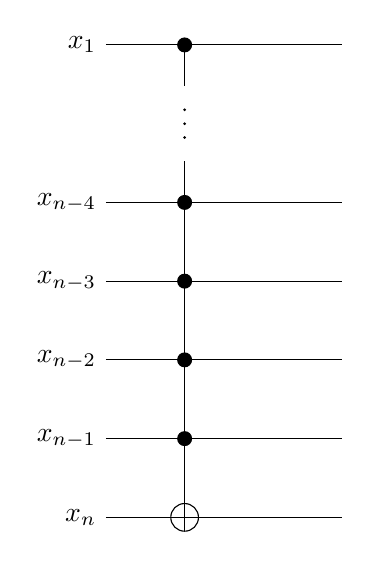
\begin{tikzpicture}
            \draw (0,6) node[anchor = east] {$x_1$} -- (3,6);
            \draw (0,4) node[anchor = east] {$x_{n-4}$} -- (3,4);
            \draw (0,3) node[anchor = east] {$x_{n-3}$} -- (3,3);
            \draw (0,2) node[anchor = east] {$x_{n-2}$} -- (3,2);
            \draw (0,1) node[anchor = east] {$x_{n-1}$} -- (3,1);
            \draw (0,0) node[anchor = east] {$x_n$} -- (3,0);
            \draw (1,-5pt) -- (1,4) --++ (0,15pt);
            \draw (1,6) --++ (0,-15pt);

            \draw (1,5) ++ (0,5pt) node [circle, draw, minimum size= 0.5pt, fill = black, inner sep=0pt, outer sep=0pt] {};
            \node at (1,5) [circle, draw, minimum size= 0.5pt, fill = black, inner sep=0pt, outer sep=0pt] {};
            \draw (1,5) ++ (0,-5pt) node [circle, draw, minimum size= 0.5pt, fill = black, inner sep=0pt, outer sep=0pt] {};

            \node at (1,0) [circle, draw, minimum size = 10pt, inner sep=0pt, outer sep=0pt] {};
            \node at (1,1) [circle, draw, minimum size= 5pt, fill = black, inner sep=0pt, outer sep=0pt] {};
            \node at (1,2) [circle, draw, minimum size= 5pt, fill = black, inner sep=0pt, outer sep=0pt] {};
            \node at (1,3) [circle, draw, minimum size= 5pt, fill = black, inner sep=0pt, outer sep=0pt] {};
            \node at (1,4) [circle, draw, minimum size= 5pt, fill = black, inner sep=0pt, outer sep=0pt] {};
            \node at (1,6) [circle, draw, minimum size= 5pt, fill = black, inner sep=0pt, outer sep=0pt] {};
          \end{tikzpicture}
        \end{figure}
        I am not sure if this is what was wanted, but it is not a very informative diagram to me.
        The classical circuit is the circuit that XORs the $n$-th bit with the AND of all the other $n-1$ bits.
        The details of the $n$-bit Toffoli gate are shown in the diagram below:
        \begin{figure}[H]
          \centering
          \begin{tikzpicture}
            \draw (0,10) node[anchor = east] {$x_1$} -- (12,10);
            \draw (0,8) node[anchor = east] {$x_2$} -- (12,8);
            \node at (2,7) [square,draw] (and1) {AND};
            \draw let \p1 = (and1.north west), \p2 = ($(and1.north west) + (-0.5,0)$) in (\p1) ++ (0,-10pt) --++ (-0.5, 0) -- (\x2, 10);
            \draw let \p1 = (and1.south west), \p2 = ($(and1.south west) + (-1,0)$) in (\p1) ++ (0,10pt) --++ (-1, 0) -- (\x2, 8);
            \node at (4,7.2) [circle,draw, fill = black, inner sep=1pt, outer sep=0pt] (dot1) {};
            \node at (4,7) [circle,draw, fill = black, inner sep=1pt, outer sep=0pt] (dot2) {};
            \node at (4,6.8) [circle,draw, fill = black, inner sep=1pt, outer sep=0pt] (dot3) {};
            \draw (0,6) node[anchor = east] {$x_{n - 3}$} -- (12,6);
            \node at (4,5) [square,draw] (and2) {AND};
            \draw let \p1 = (and1.east), \p2 = (and2.north west), \p3 = ($(and1.east)!0.5!(and2.north west)$) in (\p2 ) ++ (0,-10pt) -- (\x3,\y2 - 10pt) -- (\x3,\y1) -- (\p1);
%            \draw let \p1 = (and2.north west)in (\p1) ++ (0,-10pt) --++ (-0.3, 0) --++ (0, 1.5);
            \draw let \p1 = (and2.south west), \p2 = ($(and2.south west) + (-1,0)$) in (\p1) ++ (0,10pt) --++ (-1, 0) -- (\x2, 6);
            \draw (0,4) node[anchor = east] {$x_{n-2}$} -- (12,4);
            \node at (6,3) [square,draw] (and3) {AND};
            \draw let \p1 = (and2.east), \p2 = (and3.north west), \p3 = ($(and2.east)!0.5!(and3.north west)$) in (\p2 ) ++ (0,-10pt) -- (\x3,\y2 - 10pt) -- (\x3,\y1) -- (\p1);
            \draw let \p1 = (and3.south west), \p2 = ($(and3.south west) + (-1,0)$) in (\p1) ++ (0,10pt) --++ (-1, 0) -- (\x2, 4);
            \draw (0,2) node[anchor = east] {$x_{n-1}$} -- (12,2);
            \node at (8,1) [square,draw] (and4) {AND};
            \draw let \p1 = (and3.east), \p2 = (and4.north west), \p3 = ($(and3.east)!0.5!(and4.north west)$) in (\p2 ) ++ (0,-10pt) -- (\x3,\y2 - 10pt) -- (\x3,\y1) -- (\p1);
            \draw let \p1 = (and4.south west), \p2 = ($(and4.south west) + (-1,0)$) in (\p1) ++ (0,10pt) --++ (-1, 0) -- (\x2, 2);
            \node at (10,0) [above = -10pt, square,draw] (xor) {XOR};
            \draw let \p1 = (xor.west) in (0,0) node[anchor = east] {$x_{n}$} -- (\x1, 0);
            \draw let \p1 = (xor.east) in (\x1,0) -- (12, 0);
            \draw let \p1 = (and4.east), \p2 = (xor.north west), \p3 = ($(and4.east)!0.5!(xor.north west)$) in (\p2 ) ++ (0,-10pt) -- (\x3,\y2 - 10pt) -- (\x3,\y1) -- (\p1);
          \end{tikzpicture}
        \end{figure}
      \item
        Here is the adder:
        \begin{figure}[H]
          \centering
          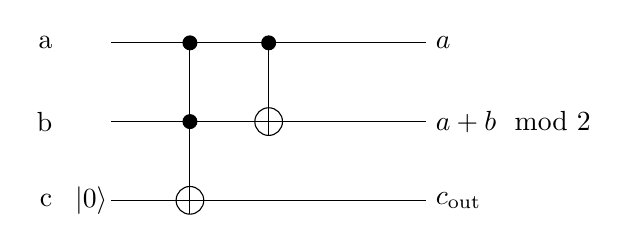
\begin{tikzpicture}
            \draw (-0,2) node[anchor = east] (a) {} -- (4,2) node[anchor = west] {$a$};
            \draw (-0,1) node[anchor = east] (b) {} -- (4,1) node[anchor = west] {$a + b \mod 2$};
            \draw (-0,0) node[anchor = east] (c) {} -- (4,0) node[anchor = west] {$c_\text{out}$};
            \draw (a) ++ (-0.5,0) node[anchor = east] {a} ;
            \draw (b) ++ (-0.5,0) node[anchor = east] {b} ;
            \draw (c) ++ (-0.5,0) node[anchor = east] {c} ;
            \draw (c) ++ (0.2,0) node[anchor = east] {$\left| 0 \right\rangle$} ;
            \draw (1,2) -- (1,-5pt);
            \node at (1,0) [circle, draw, minimum size = 10pt, inner sep=0pt, outer sep=0pt] {};
            \node at (1,1) [circle, draw, minimum size= 5pt, fill = black, inner sep=0pt, outer sep=0pt] {};
            \node at (1,2) [circle, draw, minimum size= 5pt, fill = black, inner sep=0pt, outer sep=0pt] {};
            \draw (2,2) -- (2,1) --++ (0, -5pt);
            \node at (2,2) [circle, draw, minimum size= 5pt, fill = black, inner sep=0pt, outer sep=0pt] {};
            \node at (2,1) [circle, draw, minimum size = 10pt, inner sep=0pt, outer sep=0pt] {};
          \end{tikzpicture}
        \end{figure}
        The TOFFOLI gate simply gives $(a \cdot b) \oplus 0 \equiv a \cdot b$ and the CNOT simply give $a \oplus b$ which is exactly the classical adder.
        Here is the corresponding truth table:
        \begin{figure}[H]
          \centering
          \begin{tabular} {|c|c|c||c||c|c|c|}
            \hline
            a & b & c & & a & $a + b \mod 2$ & $c_{\text{out}, (a + b)//2}$\\
            \hline
            0 & 0 & 0 & & 0 &              0 &                  0  \\
            \hline
            0 & 1 & 0 & & 0 &              1 &                  0  \\
            \hline
            1 & 0 & 0 & & 1 &              1 &                  0  \\
            \hline
            1 & 1 & 0 & & 1 &              0 &                  1  \\
            \hline
            
          \end{tabular}
        \end{figure}
      \item
        I think this question is asking for the total value of the three qubits.
        Here, a third bit must be added to the LSB of the previous circuit.
        The following circuit achieves this:
        \begin{figure}[H]
          \centering
          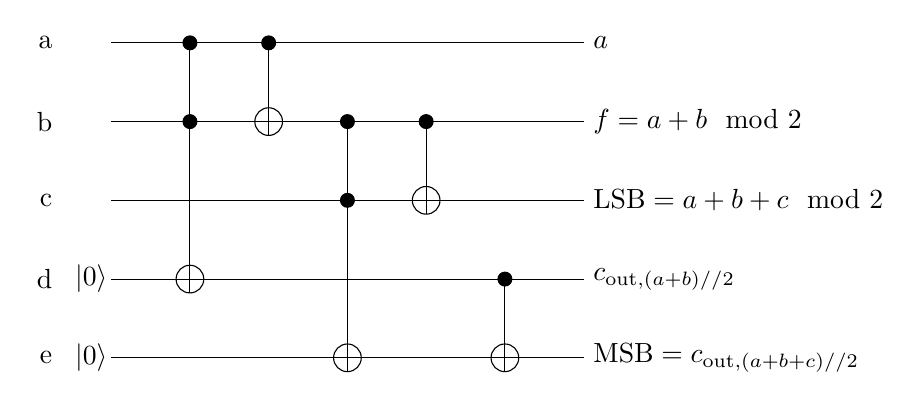
\begin{tikzpicture}
            \draw (-0,4) node[anchor = east] (a) {} -- (6,4) node[anchor = west] {$a$};
            \draw (-0,3) node[anchor = east] (b) {} -- (6,3) node[anchor = west] {$f = a + b \mod 2$};
            \draw (-0,2) node[anchor = east] (c) {} -- (6,2) node[anchor = west] {$\text{LSB} = a + b + c \mod 2$};
            \draw (-0,1) node[anchor = east] (d) {} -- (6,1) node[anchor = west] {$c_{\text{out}, (a + b)//2}$};
            \draw (-0,0) node[anchor = east] (e) {} -- (6,0) node[anchor = west] {$\text{MSB} = c_{\text{out}, (a + b + c)//2}$};
            \draw (a) ++ (-0.5,0) node[anchor = east] {a} ;
            \draw (b) ++ (-0.5,0) node[anchor = east] {b} ;
            \draw (c) ++ (-0.5,0) node[anchor = east] {c} ;
            \draw (d) ++ (-0.5,0) node[anchor = east] {d} ;
            \draw (e) ++ (-0.5,0) node[anchor = east] {e} ;
            \draw (d) ++ (0.2,0) node[anchor = east] {$\left| 0 \right\rangle$} ;
            \draw (e) ++ (0.2,0) node[anchor = east] {$\left| 0 \right\rangle$} ;

            \draw (1,4) -- (1,1) -- ++ (0,-5pt);
            \node at (1,1) [circle, draw, minimum size = 10pt, inner sep=0pt, outer sep=0pt] {};
            \node at (1,4) [circle, draw, minimum size= 5pt, fill = black, inner sep=0pt, outer sep=0pt] {};
            \node at (1,3) [circle, draw, minimum size= 5pt, fill = black, inner sep=0pt, outer sep=0pt] {};

            \draw (2,4) -- (2,3) --++ (0, -5pt);
            \node at (2,4) [circle, draw, minimum size= 5pt, fill = black, inner sep=0pt, outer sep=0pt] {};
            \node at (2,3) [circle, draw, minimum size = 10pt, inner sep=0pt, outer sep=0pt] {};

            \draw (4,3) -- (4,2) --++ (0, -5pt);
            \node at (4,3) [circle, draw, minimum size= 5pt, fill = black, inner sep=0pt, outer sep=0pt] {};
            \node at (4,2) [circle, draw, minimum size = 10pt, inner sep=0pt, outer sep=0pt] {};

            \draw (3,3) -- (3,0) -- ++ (0,-5pt);
            \node at (3,0) [circle, draw, minimum size = 10pt, inner sep=0pt, outer sep=0pt] {};
            \node at (3,3) [circle, draw, minimum size= 5pt, fill = black, inner sep=0pt, outer sep=0pt] {};
            \node at (3,2) [circle, draw, minimum size= 5pt, fill = black, inner sep=0pt, outer sep=0pt] {};

            \draw (5,1) -- (5,0) --++ (0, -5pt);
            \node at (5,1) [circle, draw, minimum size= 5pt, fill = black, inner sep=0pt, outer sep=0pt] {};
            \node at (5,0) [circle, draw, minimum size = 10pt, inner sep=0pt, outer sep=0pt] {};
          \end{tikzpicture}
        \end{figure}
        Here is the corresponding truth table:
        \begin{figure}[H]
          \centering
          \begin{tabular} {|c|c|c|c|c||c||c|c|c|c|c|c|}
            \hline
            a & b & c & d & e & & a & $a + b \mod 2$ & $\text{LSB}      $ & $c_{\text{out}, (a + b)//2}$ & $f \cdot c \oplus e         $    & $c_{\text{out}, (a + b + c)//2}$ \\
            \hline                                                                                                                         
            0 & 0 & 0 & 0 & 0 & & 0 &              0 &                  0 &                            0 &                                0 &                                0 \\
            \hline                                                                                                                         
            0 & 0 & 1 & 0 & 0 & & 0 &              0 &                  1 &                            0 &                                0 &                                0 \\
            \hline                                                                                                                         
            0 & 1 & 0 & 0 & 0 & & 0 &              1 &                  1 &                            0 &                                0 &                                0 \\
            \hline                                                                                                                         
            0 & 1 & 1 & 0 & 0 & & 0 &              1 &                  0 &                            0 &                                1 &                                1 \\
            \hline                                                                                                                         
            1 & 0 & 0 & 0 & 0 & & 1 &              1 &                  1 &                            0 &                                0 &                                0 \\
            \hline                                                                                                                         
            1 & 0 & 1 & 0 & 0 & & 1 &              1 &                  0 &                            0 &                                1 &                                1 \\
            \hline                                                                                                                         
            1 & 1 & 0 & 0 & 0 & & 1 &              0 &                  0 &                            1 &                                0 &                                1 \\
            \hline                                                                                                                         
            1 & 1 & 1 & 0 & 0 & & 1 &              0 &                  1 &                            1 &                                0 &                                1 \\
            \hline
            
          \end{tabular}
        \end{figure}
    \end{enumerate}
  \item
    \begin{enumerate}
      \item
        The circuit for the search of 000 is at this \href{https://quantum.ibm.com/composer/files/new?initial=N4IgdghgtgpiBcIBSB7MKDiKCuB3AzgLQAMpIANCAI4T5QIgDyACgKIByAigIIDKAsgAIATADpiAbgA6YAJZgAxgBtsAExiCp1GEtkAjAIyj5CrdLAyqAJxgBzQVQDaAFgC65hTfsKX7mTfwYABcHR2I-MADg0IMIqJCnYQiAC1Ck81SnWIzQ8PM9CCsrWRgrXIiCopKyrIrC4tK0iIAPcvNW2vamnKc8mQUFDsdY8ibR3pS2mUqGmuG6qsbElu6ZIey1qbAZ6q2dpfn8\%2Bt3lnsd0mUzDy62hi7B1lYmz\%2B-25vu3jg43FQfLx\%2BYA\%2B5DD5vGKTU6bTrTL7vCFhJ7neE-K6vWF7dHQz6LObA27grqQsBXD4DR5A1wAj4khazAkwnGrB5Mx6EhFHRnPBl0rFgomo5Hwj53RE-EHwtGc9nck7XX7igEjJl86XMrnYnlygVslH4-n04nKzFIjma0HGsV6uUis6kv61ClUoW02U-FV4omsqGqlXmqVu433bU3dVXS2eq26okqgNSu0K8EU02ul0HYWRiXOs7hk0h3Ma2V\%2BzWxzUe1VetX5mkee2AsZbasy76p3GIss5ouFlsG92Z22Ctll9NY4MF5vJtMRMn-RNG-3d9XinV9vPUg02vOSs0LuW9tnD61Mxvy2fLJ39idzEuysvtxGdyeXnuBleG0PrlkZl476\%2BP-q18JFUpOdix3A8DyjKsGw-fVo2NB8rx3IdRTbLN-3Jet33VGMkNQ5d9zAn9cO-C88xzZD8M3Iin3VacJiApMm0Qmjyy-KjSLfQ9YPzCgQHUfBPFkAAHIJZDQBgQAAXyAA}{link}.
        The number of repetitions that maximises the amplitude seems to be six, but I am not sure how to show this analytically.
%        The initial state is:
%        \begin{equation*}
%          \left| s \right\rangle = \hat H^{\otimes 3} \left| 00 \right \rangle
%        \end{equation*}
%        Amplitude inversion and amplification operator is:
%        \begin{align*}
%          \left| s \right\rangle \left\langle s \right| &= 2 \hat H^{\otimes 3} \left| 00 \right \rangle \left\langle 00 \right|\hat H^{\otimes 3} - I \\
%                                                        &= \hat H^{\otimes 3} \text{NOT}^{\otimes 3} (I \otimes I \otimes \hat H) \text{TOFFOLI} (I \otimes I \otimes \hat H) \text{NOT}^{\otimes 3}  \hat H^{\otimes 3}
%        \end{align*}
%        The oracle is:
      \item
        The circuit for the search of both 011 and 101 is at this \href{ https://quantum.ibm.com/composer/files/new?initial=N4IgdghgtgpiBcIBSB7MKDiKCuB3AzgLQAMAjKQGSlkgA0IAjhPlAiAPIAKAogHICKAQQDKAWQAEAJgB0xANwAdMAEswAYwA22ACYxxCxjA3KARqWmq1BxWCUMATjADm4hgG0ALAF0baxy7VPHyVHfBgAF1c3YmCwUIio0lj4yPdJWIALKPSbLPck3KiYmxMIe3tlGHsi2NLyyur82rKKquzYtQAvGtpE5vq2tI7uod6mkpaGmomBxuj\%2B1rmCpTrF9sKhjfmt5bAAD3WlA-dio76tnJXJwbdd1amTjrVj\%2BbHbrzfLsHubu\%2Bu5077aZncZKPJuL7gwHg3YvSGHMB0EC6fB\%2BZQAB3CyjQbBAAF8gA}{link}.
      \item
        The circuit for the search of both 011 and 101 is at this \href{https://quantum.ibm.com/composer/files/new?initial=N4IgdghgtgpiBcIBSB7MKDiKCuB3AzgLQAMAjKcQDQXFUUUBk5tIlIAjhPlAiAPIAFAKIA5AIoBBAMoBZAAQAmAHTEA3AB0wASzABjADbYAJjDnqOMfVoBGpJTt3mNYTewBOMAOZz2AbQAsALrOuh7eugHBmgAWPr7EUWCxfqSJyb4KaXEAzInWEG5uWjBucQnO\%2BYXFpSl5BUUlcZkV9dU5iQAeZXVVjbUtvTUZPQ1DuSHZXX4JlHGps36ZC77jmroAXt3Lq3qTW3OBy0vtzlPxI239mpWjTRd9K-dD5detD6kDt4tPJzG-Sd1nOkPn9vqd-mcXmAziDoXcgf8bpdzp9kbCkQ9mms9tNDgcjni-DsMc8flcwCT4ZpIZ0DuCwaDHgjcczfLD0li4USstznKwQCZ8KEtAAHAAuWjQvBAAF8gA}{link}.
%        \begin{listings}
%x q[0];
%x q[1];
%x q[2];
%h q[0];
%ccx q[1], q[2], q[0];
%h q[0];
%barrier q[1];
%barrier q[2];
%x q[2];
%x q[1];
%x q[0];
%barrier q[0];
%barrier q[1];
%barrier q[2];
%h q[2];
%barrier q[1];
%barrier q[0];
%h q[0];
%h q[1];
%x q[2];
%x q[0];
%x q[1];
%h q[2];
%ccx q[0], q[1], q[2];
%x q[0];
%x q[1];
%h q[2];
%h q[0];
%h q[1];
%x q[2];
%h q[2];
%        \end{listings}
%        Four bit oracle
%        \begin{listings}
%OPENQASM 2.0;
%include "qelib1.inc";
%
%qreg q[4];
%creg c[4];
%h q[0];
%h q[1];
%h q[2];
%h q[3];
%barrier q[0];
%barrier q[1];
%barrier q[2];
%barrier q[3];
%x q[0];
%c3x q[0], q[1], q[2], q[3];
%x q[0];
%barrier q[3];
%barrier q[1];
%barrier q[2];
%x q[2];
%x q[3];
%x q[1];
%x q[0];
%barrier q[2];
%x q[3];
%barrier q[1];
%barrier q[0];
%cz q[0], q[3];
%barrier q[0];
%x q[3];
%barrier q[1];
%barrier q[2];
%x q[0];
%x q[3];
%x q[1];
%x q[2];
%x q[0];
%c3x q[0], q[1], q[2], q[3];
%x q[0];
%barrier q[1];
%barrier q[2];
%barrier q[3];
%barrier q[0];
%barrier q[1];
%barrier q[2];
%barrier q[3];
%        \end{listings}

    \end{enumerate}
\end{enumerate}
\end{document}
